\documentclass[UTF8,a4paper,12pt]{ctexart}

\usepackage{geometry}
\usepackage{graphicx}
\usepackage{booktabs}
\usepackage{longtable}
\usepackage{tabularx}
\usepackage{array}
\usepackage{enumitem}
\usepackage{xcolor}
\usepackage{hyperref}
\usepackage{caption}
\usepackage{float}
\usepackage{amsmath}
\usepackage{listings}
\usepackage{tikz}
\usetikzlibrary{arrows.meta,positioning}

\geometry{left=2.6cm,right=2.6cm,top=2.6cm,bottom=2.6cm}
\graphicspath{{../../}{./}}
\hypersetup{
  colorlinks=true,
  linkcolor=blue!50!black,
  urlcolor=blue!55!black,
  citecolor=blue!50!black
}
\setlist[itemize]{leftmargin=2em,itemsep=0.2em,topsep=0.3em}
\setlist[enumerate]{leftmargin=2em,itemsep=0.2em,topsep=0.3em}
\captionsetup{font=small,labelfont=bf}
\renewcommand{\arraystretch}{1.25}
\lstset{
  basicstyle=\ttfamily\small,
  breaklines=true,
  frame=single,
  columns=fullflexible,
  backgroundcolor=\color{gray!6}
}

\newcolumntype{Y}{>{\raggedright\arraybackslash}X}
\newcommand{\code}[1]{\texttt{#1}}

\title{\textbf{工业轴承设备剩余寿命预测项目技术报告}}
\author{中国科学技术大学软件学院《软件工程》课程项目\\指导老师：zjf\\小组成员：zyj、cyy、zdh、zy}
\date{2026 年 6 月}

\begin{document}
\maketitle

\begin{abstract}
本报告面向“工业轴承设备剩余寿命预测系统的实现”课程项目，对现有代码、文档、实验结果和答辩材料进行统一技术整理。项目面向预测性维护场景，以 XJTU-SY 与 PHM2012/FEMTO 两类真实轴承退化数据为主要对象，完成数据加载、时间语义整理、信号预处理、19 维时频域特征提取、RUL 标签构造、模型训练、指标评价、复现实验证据和课程材料归档。需求分析中明确两类预测目标：一类是 RUL 数值预测，回答“还能运行多久”；另一类是生存概率或失效风险估计，回答“未来某一时间范围内失效风险多高”。当前技术主线为 RUL 回归预测流程，生存分析与失效概率保留为扩展能力和补充证据。报告采用保守口径描述当前完成度：项目已形成可运行、可测试、可复查的 RUL 预测流程，但不宣称生产级失效概率预测能力，也不宣称全部外部 SOTA 已本地复现完成。
\end{abstract}

\noindent\textbf{关键词：}预测性维护；滚动轴承；剩余寿命预测；RUL；生存概率；特征工程；深度学习；软件工程

\newpage
\tableofcontents
\newpage

\section{项目概述}

\subsection{问题背景}

滚动轴承是旋转机械中的关键部件，其退化会直接影响设备安全、生产连续性和维护成本。传统事后维修容易造成突发停机，定期维修又可能导致过早维护和资源浪费。预测性维护希望在设备失效前识别退化趋势，并估计剩余可用寿命，从而为检修计划提供依据。

本项目围绕轴承振动数据实现一个课程范围内可运行、可测试、可复查的剩余寿命预测流程。它不是单个算法脚本，而是把数据接入、特征构造、标签生成、模型训练、指标评价、实验记录、图表展示和文档归档组织为一条工程化链路。项目主命名空间为 \code{USTC.SSE.BearingPrediction}，环境管理使用 \code{uv}，核心代码位于 \code{src/USTC/SSE/BearingPrediction}。

\subsection{预测目标与完成口径}

项目需求中包含两类建模输出：

\begin{enumerate}
  \item \textbf{基于时间序列的 RUL 回归预测。}输出连续剩余寿命值，用 RMSE、MAE、Score 等指标评价。
  \item \textbf{基于生存分析的失效概率建模。}输出生存概率或风险率，用 C-index、Brier Score 等指标评价。
\end{enumerate}

当前实现与验证应按“主线 + 扩展”解释。主线是 RUL 回归预测，已经形成从真实数据到预测文件和指标表的闭环；生存概率和失效概率是扩展能力，代码中保留 Kaplan-Meier、Cox 等基础接口，并在 RULSurv RSF port 中补充了与概率解码相关的证据，但尚未作为与两篇 RUL 论文复现同等规格的主验收实验展开。

\subsection{总体完成内容}

\begin{table}[H]
\centering
\caption{项目完成内容概览}
\begin{tabularx}{\textwidth}{p{3.0cm}Y}
\toprule
类别 & 完成内容 \\
\midrule
需求分析 & 明确预测性维护场景、输入输出、RUL 数值预测和失效风险概率两个目标。 \\
数据接入 & 支持 XJTU-SY、PHM2012/FEMTO 和合成数据，统一输出 \code{BearingEntity}。 \\
特征工程 & 实现 14 个时域特征和 5 个频域特征，共 19 维，并生成可解释特征趋势图。 \\
标签构造 & 支持原始窗口 RUL 标签、特征序列 RUL 标签和退化阶段标签。 \\
模型训练 & 支持 CNN、RNN、MLP、Transformer、CNN-LSTM-AM、XLSTM-Transformer 等模型。 \\
预测方式 & 支持直接预测、滚动预测和 MC Dropout 不确定性估计。 \\
概率扩展 & 保留生存分析服务，支持 Kaplan-Meier、Cox 生存概率和失效概率输出。 \\
实验验证 & 完成 CNN-LSTM-AM 与 xLSTM-Transformer 两篇 RUL 论文的工程化复现。 \\
测试材料 & 全量 \code{pytest} 当前为 59 个测试通过，8 个 notebook 纳入示例验收。 \\
\bottomrule
\end{tabularx}
\end{table}

\section{需求分析}

\subsection{用户与场景}

项目面向三个层面的使用者。第一类是实验开发者，他们关心数据能否导入、特征和标签是否构造正确、训练流程是否可复跑。第二类是课程评审人员，他们关心项目是否真实实现、是否可运行、是否有测试和文档支撑。第三类是后续维护者，他们关心是否能替换数据集、替换模型或扩展概率分析。

\begin{table}[H]
\centering
\caption{使用者、关注点与项目证据}
\begin{tabularx}{\textwidth}{p{3.2cm}Y Y}
\toprule
使用者 & 关注问题 & 项目提供的证据 \\
\midrule
实验开发者 & 数据和特征是否可复查 & loader、labeler、notebook、pytest、CSV 输出。 \\
课程评审人员 & 是否真实完成工程流程 & 训练历史、预测表、指标表、测试报告、结题材料。 \\
后续维护者 & 是否便于扩展 & 分层模块、公开 API、统一实体、脚本和文档。 \\
\bottomrule
\end{tabularx}
\end{table}

\subsection{输入输出需求}

项目输入是按时间顺序保存的轴承 run-to-failure 振动快照。当前主线使用水平、垂直振动通道，PHM2012/FEMTO 中的温度通道由 loader 保留，作为后续多源融合扩展。

项目输出分为两类：

\begin{itemize}
  \item \textbf{RUL 数值输出。}直接给出当前样本或特征序列对应的剩余寿命值，并生成预测曲线、真实值/预测值表和回归误差指标。
  \item \textbf{概率输出。}通过生存分析或 RULSurv 风格实验输出给定 horizon 或给定生存概率阈值下的失效风险解释。该部分是扩展能力，不作为结题主验收路线。
\end{itemize}

RUL 值与失效概率描述的是同一退化问题的不同侧面。RUL 回答“还能运行多久”，生存概率回答“未来某一时刻前仍未失效的概率”。通常 RUL 越短，失效风险越高；但二者不是简单线性换算关系，也不应在报告中互相替代。

\subsection{功能需求}

\begin{longtable}{p{2.2cm}p{4.2cm}p{8.0cm}}
\caption{主要功能需求}\\
\toprule
编号 & 功能 & 技术落实 \\
\midrule
\endfirsthead
\toprule
编号 & 功能 & 技术落实 \\
\midrule
\endhead
FR-1 & 数据接入与管理 & \code{XJTULoader}、\code{PHM2012Loader}、\code{SyntheticBearingFactory}，统一输出 \code{BearingEntity}。 \\
FR-2 & 预处理与窗口切分 & \code{PreprocessingPipeline} 组合 \code{RobustClip}、\code{ZScoreNormalize}/\code{MinMaxNormalize} 和 \code{SlidingWindowSegmenter}；高层 labeler 默认启用鲁棒裁剪与 Z-score，归一化方式、窗口大小和步长可配置。 \\
FR-3 & 特征提取 & \code{SignalFeatureExtractor} 输出 19 维时频域特征，特征后端可扩展到 \code{tsfresh} 自动特征。 \\
FR-4 & 标签构造 & \code{BearingRulLabeler}、\code{FeatureSequenceRulLabeler}、\code{BearingStageLabeler}、\code{HealthIndicatorLabeler}。 \\
FR-5 & 模型训练 & \code{BaseTrainer} 统一训练 PyTorch 模型，支持回调、验证集、梯度裁剪和实验记录。 \\
FR-6 & 预测输出 & \code{DirectPredictor}、\code{RollingPredictor}、\code{MonteCarloDropoutPredictor}。 \\
FR-7 & 评价指标 & MAE、RMSE、NormalizedRMSE、SMAPE、R2、Huang RUL Score、PHM2012 Score、方向性指标。 \\
FR-8 & 可视化与报告 & 输出预测曲线、退化阶段图、注意力热图、特征趋势图和课程材料。 \\
FR-9 & 生存概率扩展 & \code{SurvivalAnalysisService} 支持 Kaplan-Meier、Cox、生存概率曲线和失效概率输出。 \\
\bottomrule
\end{longtable}

\section{数据集与时间语义}

\subsection{数据集概况}

项目主要使用 XJTU-SY 与 PHM2012/FEMTO 两类公开轴承退化数据。二者都属于 run-to-failure 数据，适合做 RUL 预测和健康趋势分析，但文件组织、快照长度和时间语义不同。

\begin{table}[H]
\centering
\caption{XJTU-SY 与 PHM2012/FEMTO 数据差异}
\begin{tabularx}{\textwidth}{p{3.2cm}Y Y}
\toprule
项目 & XJTU-SY & PHM2012/FEMTO \\
\midrule
采样频率 & 25.6 kHz & 25.6 kHz \\
单快照点数 & 32768 & 2560 \\
单快照覆盖时长 & 约 1.28 s & 约 0.1 s \\
相邻快照间隔 & 约 60 s & 约 10 s \\
通道 & 水平、垂直振动 & 水平、垂直振动，另有温度文件 \\
组织方式 & 三工况、多轴承完整寿命序列 & Learning/Test/Full\_Test 等竞赛语义 \\
\bottomrule
\end{tabularx}
\end{table}

这里必须区分快照覆盖时长和相邻快照间隔。前者决定单个文件内部信号长度和 FFT 分辨率；后者决定 \code{elapsed\_seconds} 和秒级 RUL 标签。若只按文件编号或抽样序号构造标签，则只能称为快照级 RUL，不应误写成真实秒级寿命。

\subsection{统一实体}

\code{BearingEntity} 是数据层向后续模块提供的统一抽象，包含 \code{entity\_id}、\code{dataset\_name}、\code{samples}、\code{sample\_rate} 和 \code{metadata}。其中 \code{samples} 保存按时间顺序排列的快照表，常见列包括 \code{sample\_index}、\code{timestamp}、\code{rul}、水平振动、垂直振动、温度通道和原始文件名。

loader 的职责是把数据集差异限制在读取层。模型训练代码不直接理解 XJTU-SY 或 PHM2012 的目录结构，而是消费整理后的实体、特征表和标签。

\begin{figure}[H]
\centering
\resizebox{\textwidth}{!}{%
\begin{tikzpicture}[
  node distance=0.8cm and 0.9cm,
  box/.style={draw=blue!55!black, rounded corners=2pt, align=center, fill=blue!4, minimum width=3.4cm, minimum height=0.95cm, font=\small},
  process/.style={draw=gray!70!black, rounded corners=2pt, align=center, fill=gray!6, minimum width=3.8cm, minimum height=0.95cm, font=\small},
  target/.style={draw=green!45!black, rounded corners=2pt, align=center, fill=green!6, minimum width=3.4cm, minimum height=0.95cm, font=\small},
  note/.style={draw=orange!70!black, dashed, rounded corners=2pt, align=center, fill=orange!8, minimum width=3.8cm, minimum height=0.95cm, font=\small},
  arrow/.style={-{Latex[length=2mm]}, line width=0.45pt},
  dashedarrow/.style={-{Latex[length=2mm]}, dashed, line width=0.45pt}
]
\node[box] (source) {XJTU-SY\\PHM2012/FEMTO\\CSV/合成数据};
\node[process, right=of source] (loader) {Loader / Factory\\解析文件、时间戳、\texttt{rul}\\不做随机右删失};
\node[process, right=of loader] (entity) {\texttt{BearingEntity.samples}\\信号通道 / \texttt{sample\_index}\\\texttt{timestamp} / \texttt{rul}};

\node[target, below left=1.0cm and 0.15cm of entity] (rultarget) {RUL 回归目标\\\texttt{y = rul}};
\node[target, below right=1.0cm and 0.15cm of entity] (survtarget) {生存分析输入表\\\texttt{duration/event}\\由数据准备或实验协议提供};
\node[process, below=of rultarget] (rulmodel) {RUL 回归模型\\输出 RUL 数值};
\node[process, below=of survtarget] (survmodel) {生存分析模型\\输出 \texttt{S(t)} 与 \texttt{1-S(t)}};
\node[note, right=of survtarget] (censor) {仅 RULSurv 训练/复现实验\\25\% 随机右删失\\生成部分 \texttt{event=0}};

\draw[arrow] (source) -- (loader);
\draw[arrow] (loader) -- (entity);
\draw[arrow] (entity) -- (rultarget);
\draw[arrow] (entity) -- (survtarget);
\draw[arrow] (rultarget) -- (rulmodel);
\draw[arrow] (survtarget) -- (survmodel);
\draw[dashedarrow] (survtarget) -- (censor);
\draw[dashedarrow] (censor) |- (survmodel);
\end{tikzpicture}}
\caption{数据接入、RUL 目标与生存分析目标的关系}
\end{figure}

需要特别说明的是，随机右删失不是 \code{XJTULoader} 或 \code{PHM2012Loader} 的数据接入行为。接入层负责解析目录、快照时间、信号通道和 \code{rul} 语义；RULSurv RSF port 中的 25\% 随机右删失属于训练与复现实验协议，用于模拟部分样本未观测到失效终点的 survival setting。

\subsection{RUL 标签语义}

对完整寿命序列，RUL 的基本公式为：

\[
  RUL_i = T_{\text{end}} - t_i
\]

其中 \(t_i\) 是当前快照的运行时间，\(T_{\text{end}}\) 是该轴承最后有效快照对应的时间。XJTU-SY 可按分钟级快照间隔换算，PHM2012/FEMTO 可按约 10 秒快照间隔换算；PHM2012 Test\_set 的终止 RUL 需要结合官方条目，不能简单把本地文件末尾当作真实失效点。

\subsection{特征观察}

项目采用代表曲线和多轴承摘要共同解释退化趋势。代表曲线选取 XJTU-SY Bearing1\_1 与 PHM2012 Bearing1\_1，展示 RMS 和峰值随寿命推进的变化。这里优先使用物理含义清楚的单项特征，而不把临时合成的健康指标作为主要证据。多轴承摘要对代表轴承均匀抽样 80 个快照，比较前 20\% 与后 20\% 的特征差异。

\begin{figure}[H]
\centering
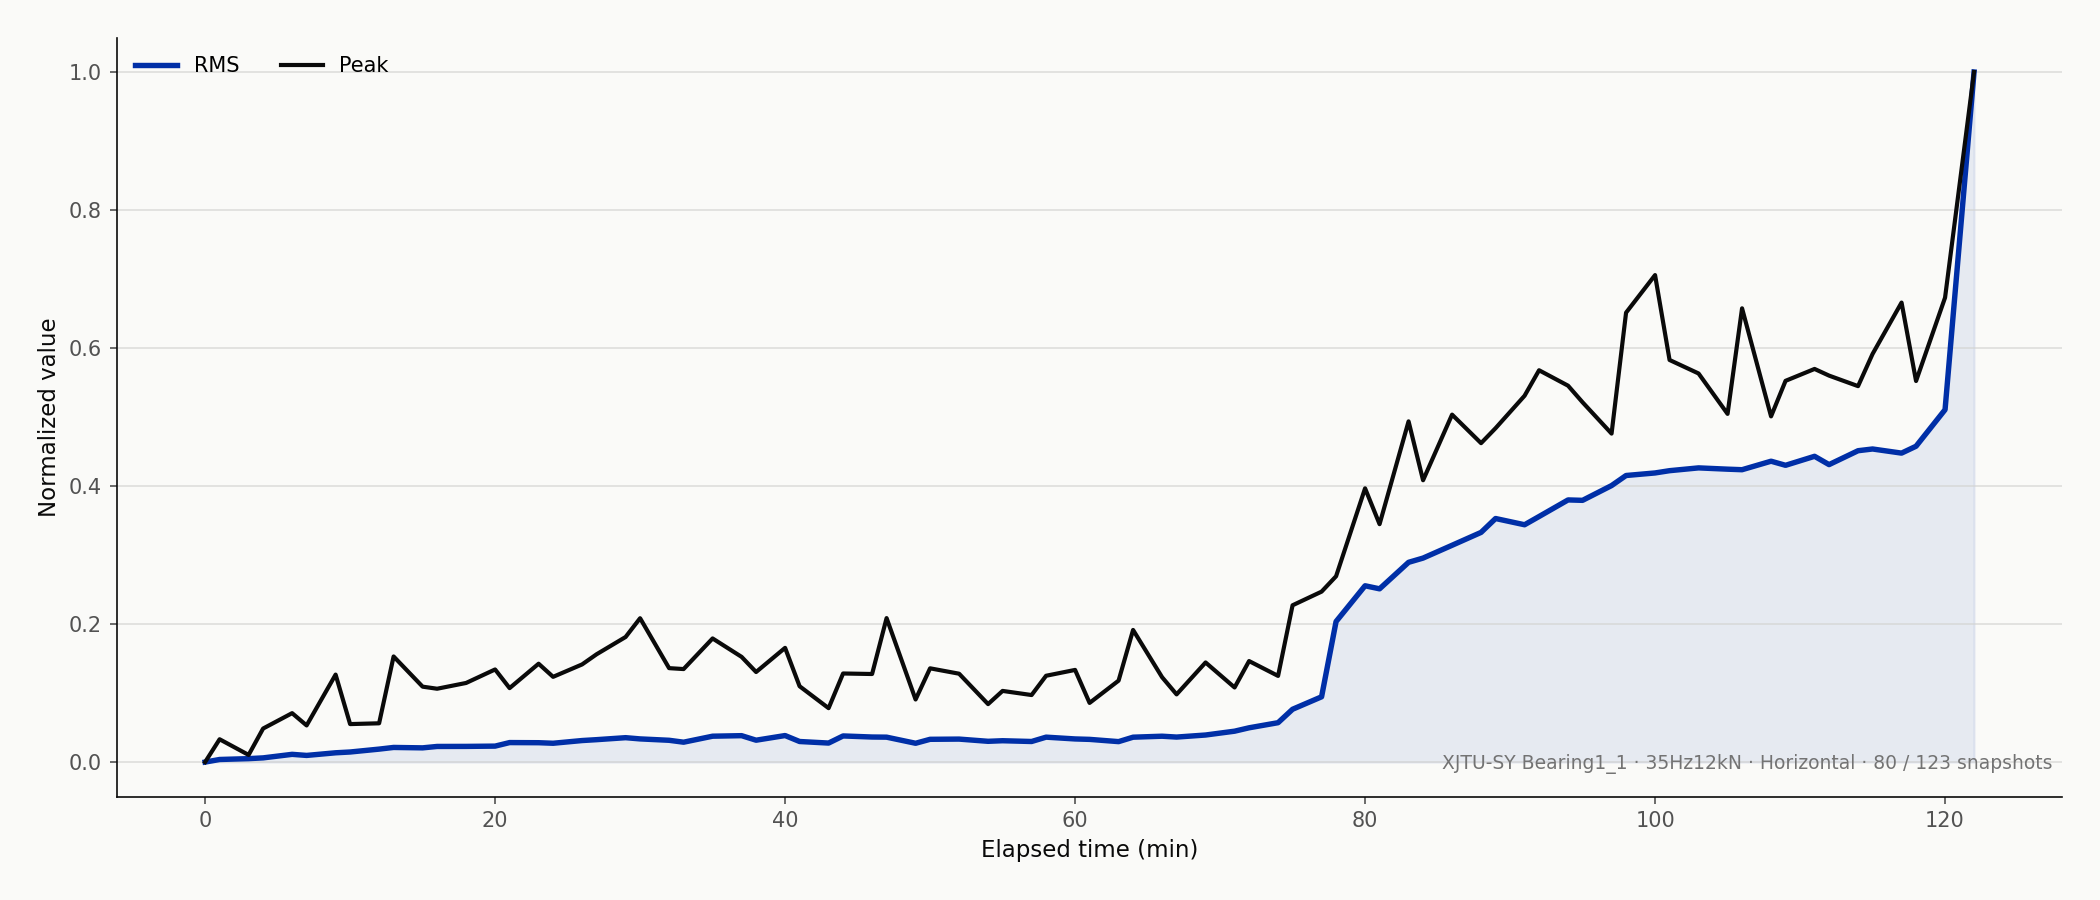
\includegraphics[width=0.92\textwidth]{docx/final/web-ppt/images/05-xjtu-bearing1-1-rms-health.png}
\caption{XJTU-SY Bearing1\_1 RMS 与峰值代表曲线}
\end{figure}

\begin{figure}[H]
\centering
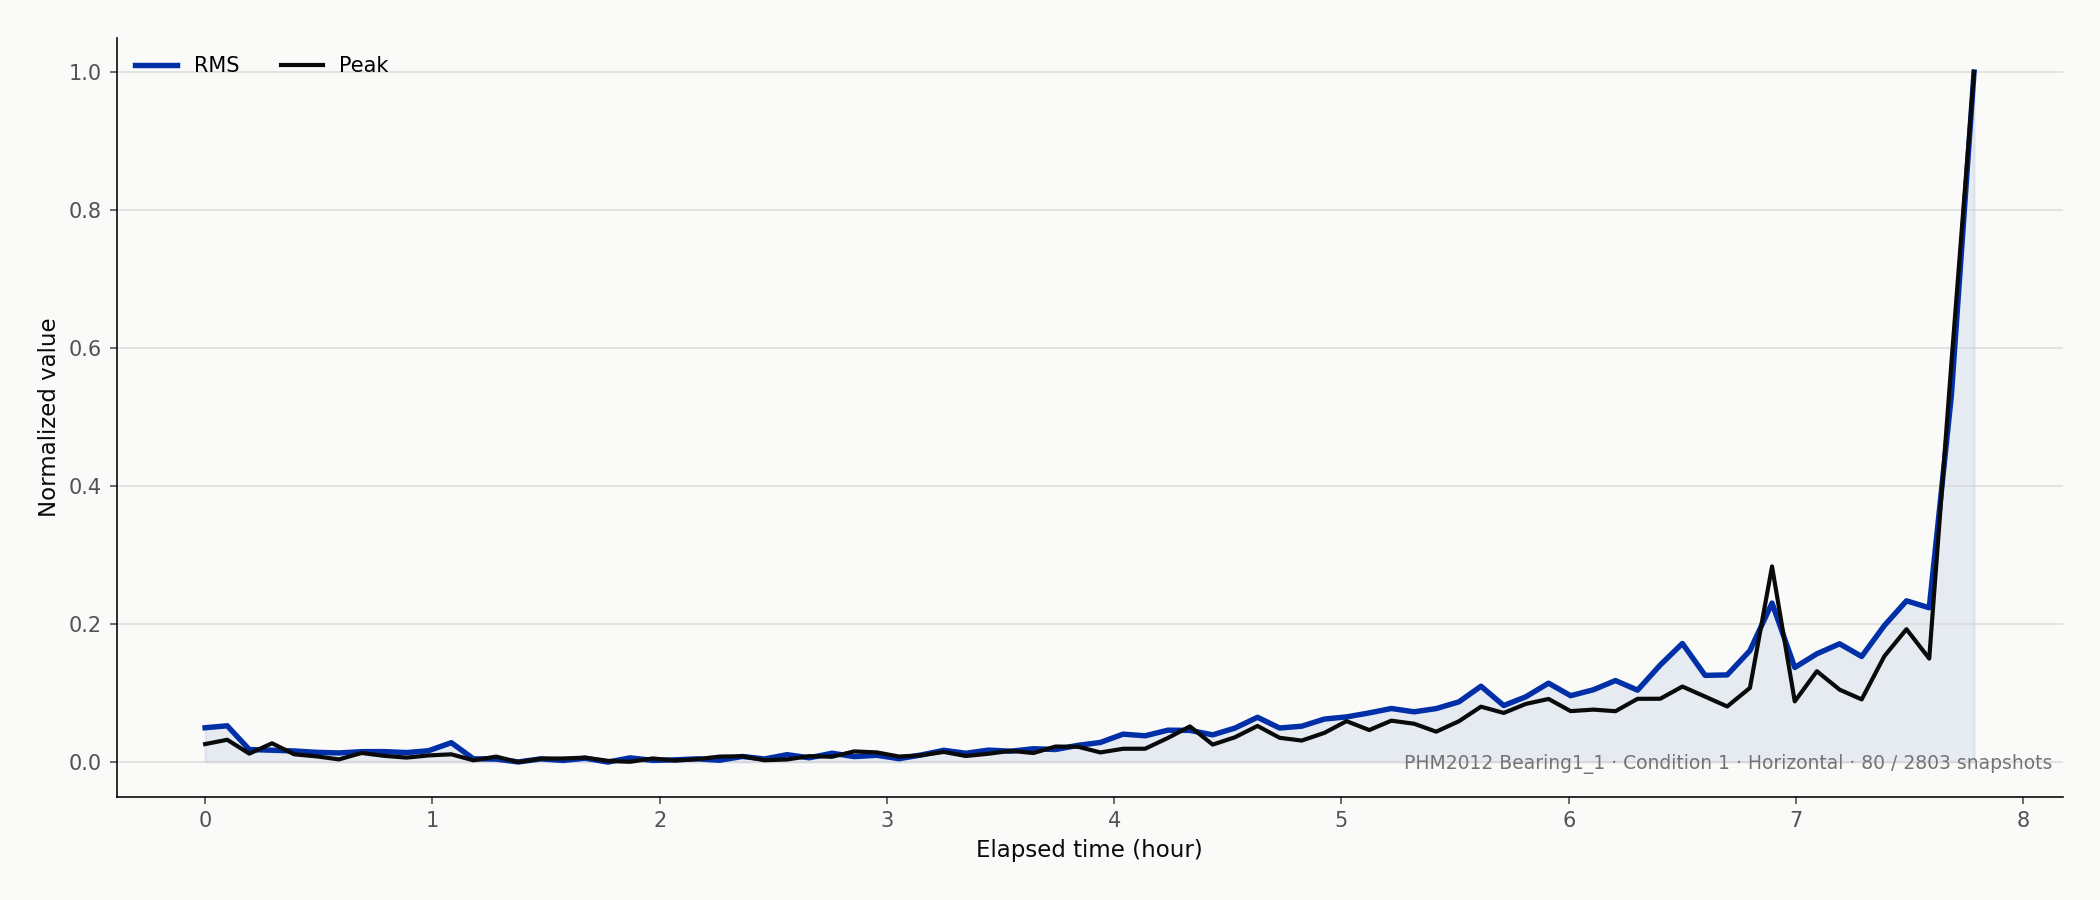
\includegraphics[width=0.92\textwidth]{docx/final/web-ppt/images/06-phm2012-bearing1-1-rms-health.png}
\caption{PHM2012 Bearing1\_1 RMS 与峰值代表曲线}
\end{figure}

\begin{figure}[H]
\centering
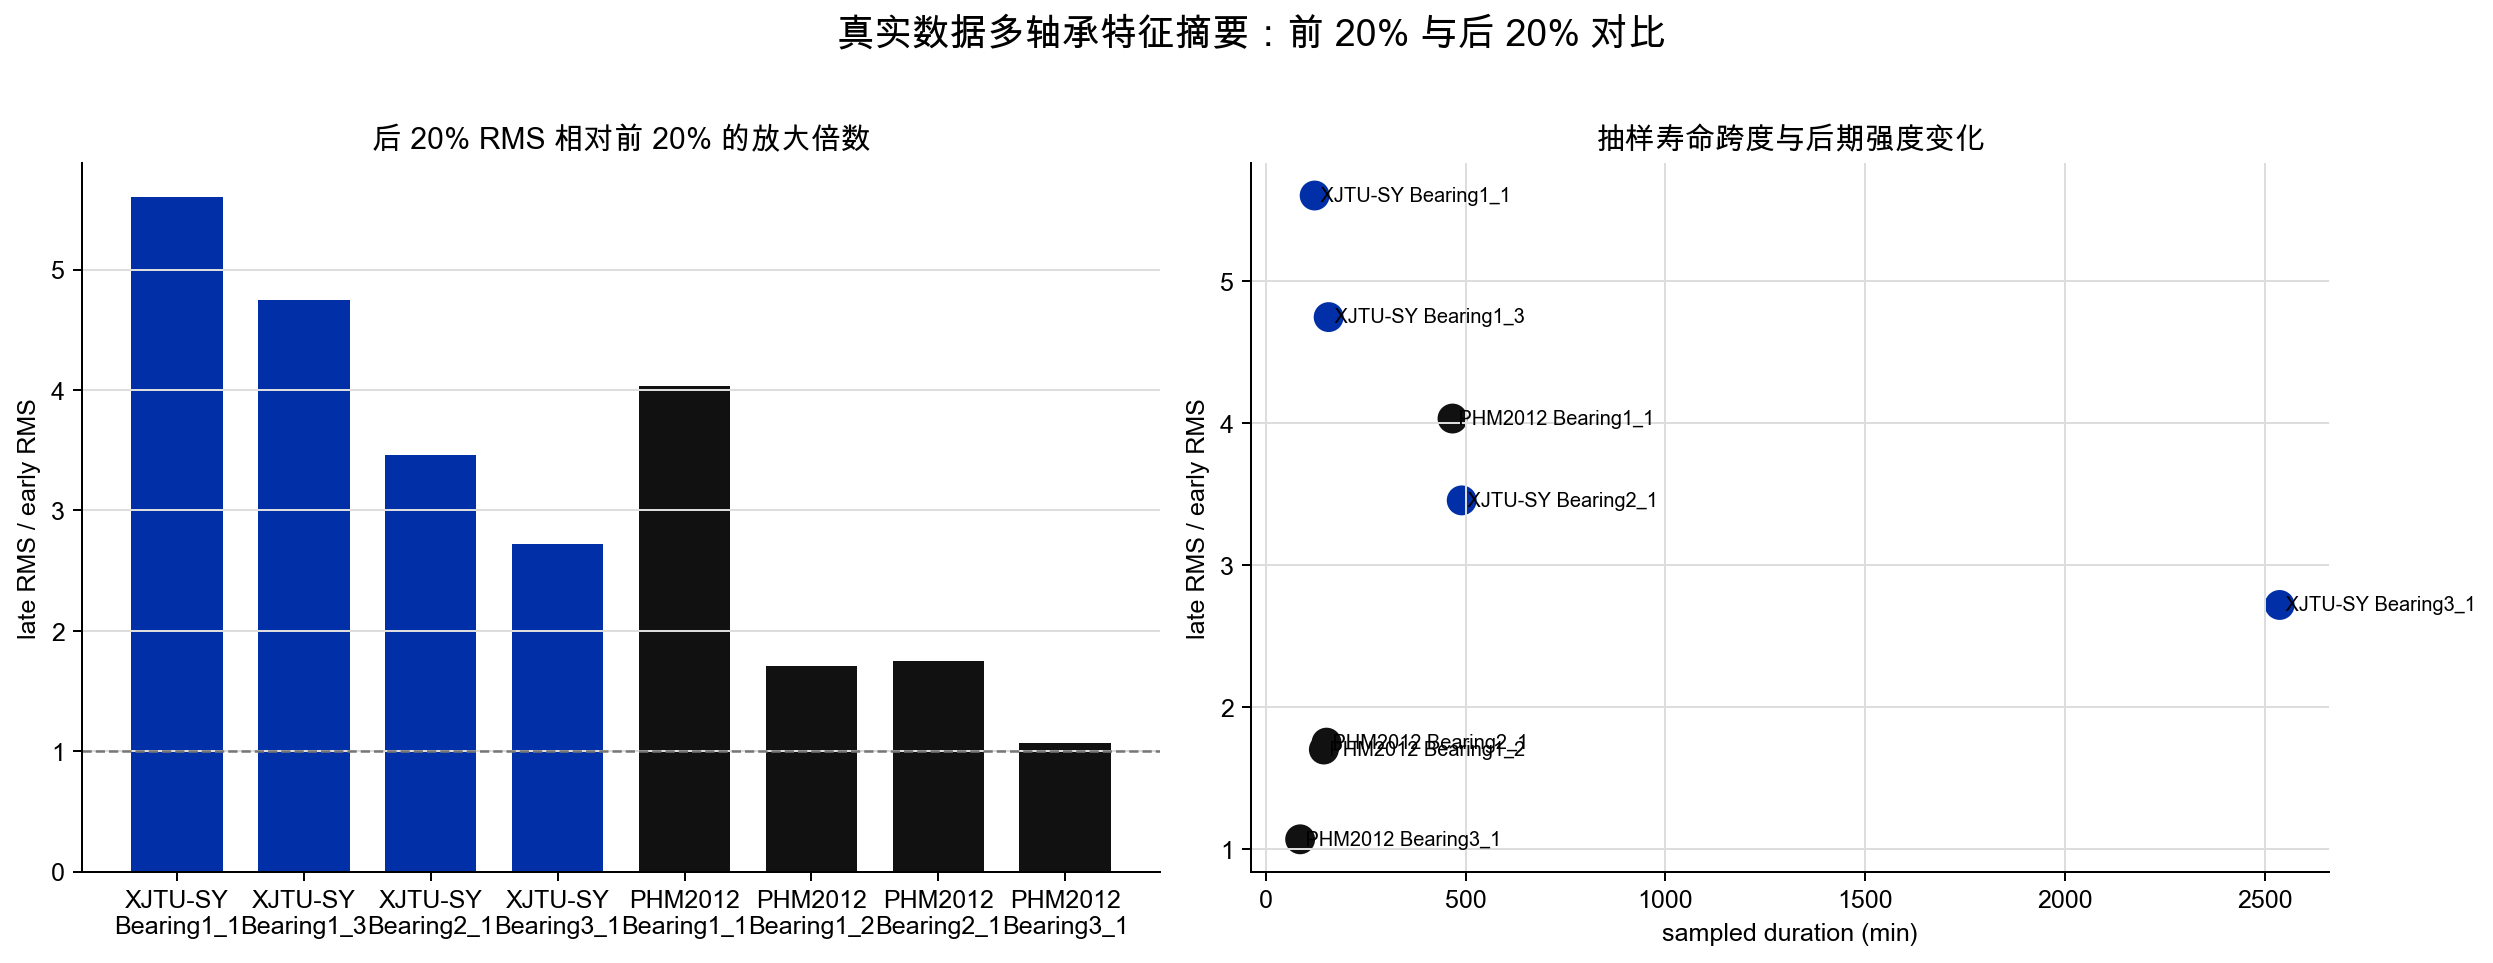
\includegraphics[width=0.92\textwidth]{docs/project-owner/assets/multi-bearing-feature-summary.png}
\caption{多轴承特征摘要}
\end{figure}

多轴承统计显示，XJTU-SY 的代表轴承后期 RMS 多数显著高于早期，谱能量放大更明显；PHM2012 也存在后期增强，但不同工况和不同轴承差异更大。这说明代表曲线可以解释特征含义，但不能替代全数据统计结论。

\section{总体技术架构}

\subsection{分层设计}

项目按数据流组织为数据层、处理层、模型层、训练层、评价层和展示层。设计原则是：loader 不训练模型，模型不读取原始文件，评价器只消费目标值和预测值，文档与图表从已有输出中提取证据。

\begin{figure}[H]
\centering
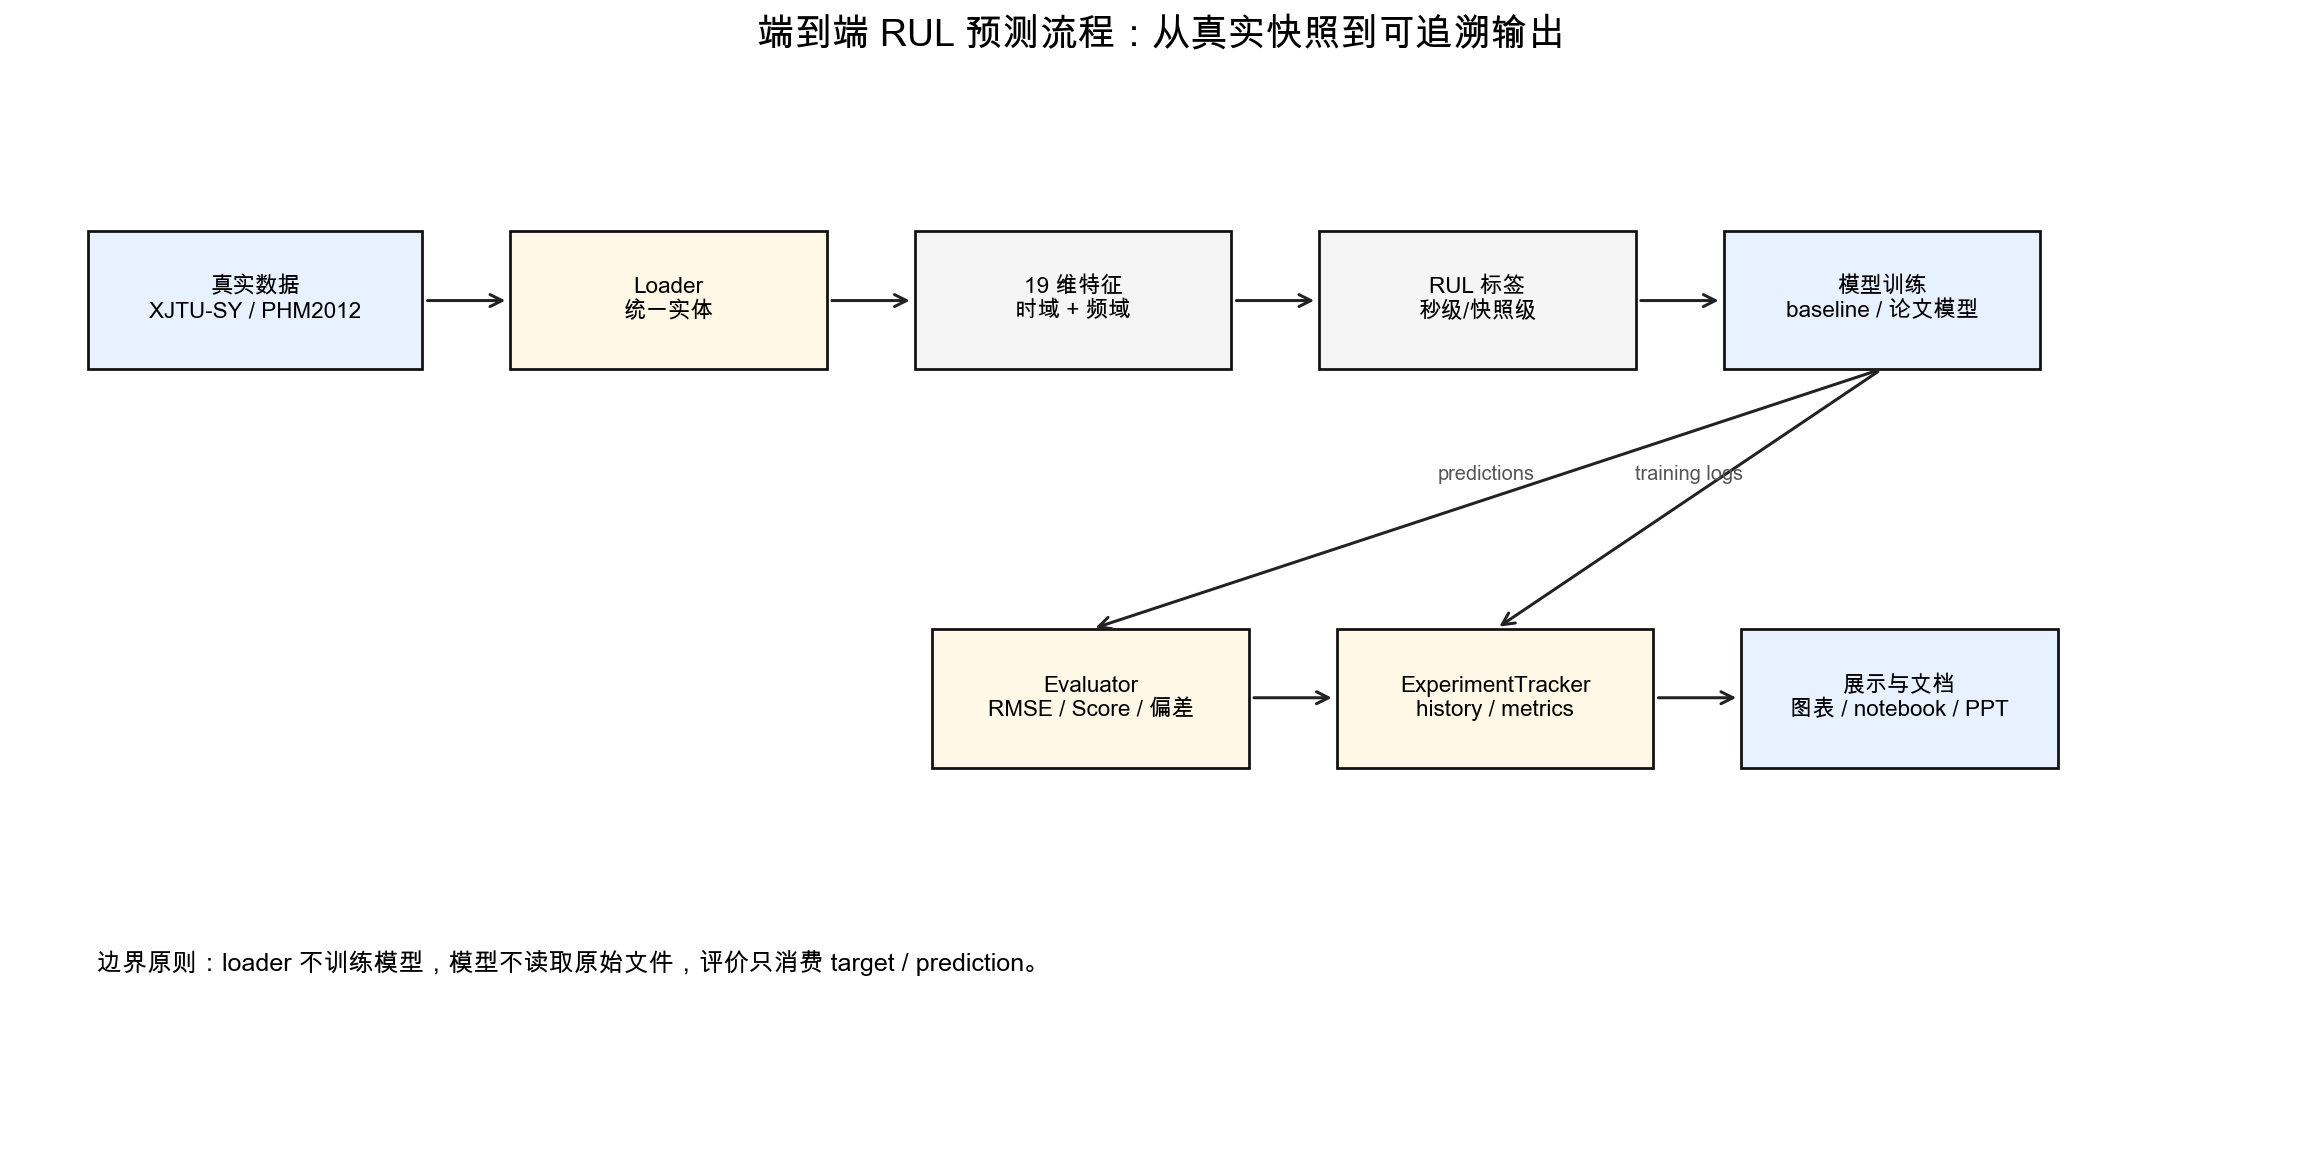
\includegraphics[width=0.95\textwidth]{docs/project-owner/assets/end-to-end-rul-architecture.png}
\caption{端到端 RUL 预测流程}
\end{figure}

\begin{table}[H]
\centering
\caption{模块边界}
\begin{tabularx}{\textwidth}{p{3.0cm}p{4.2cm}Y}
\toprule
层次 & 模块 & 职责 \\
\midrule
数据层 & \code{dataset}、\code{data} & 扫描目录、读取快照、构造统一实体和样本表。 \\
处理层 & \code{preprocess}、\code{feature}、\code{labeling} & 信号预处理、特征提取、RUL 与退化阶段标签构造。 \\
模型层 & \code{models}、\code{model} & PyTorch 模型和传统 RUL 回归模型。 \\
训练层 & \code{training}、\code{prediction} & 训练、测试、直接预测、滚动预测、不确定性估计和实验记录。 \\
评价层 & \code{evaluation} & 普通误差、RUL score、方向性偏差和分类准确率。 \\
展示层 & \code{visualization}、\code{examples}、\code{scripts} & 图表、notebook、复现脚本、课程材料生成。 \\
\bottomrule
\end{tabularx}
\end{table}

\subsection{运行入口}

\begin{table}[H]
\centering
\caption{三类运行入口}
\begin{tabularx}{\textwidth}{p{3.7cm}p{3.6cm}Y}
\toprule
入口 & 数据来源 & 作用 \\
\midrule
\code{uv run python main.py} & 合成数据 & 快速验证 API、训练、测试和可视化链路。 \\
\code{examples/*.ipynb} & demo 或真实数据 & 用户学习入口，8 个 notebook 纳入 smoke test。 \\
\code{scripts/run\_*.py} & \code{data/external} 真实数据 & 论文复现、tsfresh/sktime baseline、SOTA 证据生成；综合 workflow 位于 \code{examples/demo\_workflows.py}。 \\
\bottomrule
\end{tabularx}
\end{table}

\section{核心算法与实现}

\subsection{预处理与特征工程}

预处理层不是固定必须全部执行的黑箱，而是由 \code{PreprocessingPipeline} 串联若干 transform。其依据和可选性如下：

\begin{itemize}
  \item \textbf{鲁棒裁剪。}\code{RobustClip} 使用中位数和 MAD 对异常冲击值做裁剪，目的是降低单点异常对 RMS、峰值、峭度等特征的影响。当前高层 labeler 默认启用该步骤，但它应理解为默认工程策略，而不是数据接入层的强制语义。
  \item \textbf{幅值归一化。}\code{ZScoreNormalize} 用于消除不同轴承、通道或工况下幅值尺度差异，是当前默认选项；\code{MinMaxNormalize} 是已注册的替代选项，适合需要把输入限制到固定区间的模型。归一化方式通过 \code{normalization} 参数选择。
  \item \textbf{滑动窗口切分。}\code{SlidingWindowSegmenter} 把长振动信号切成固定长度输入，依据是 CNN、RNN、Transformer 等模型需要统一形状的张量。窗口大小和步长由 \code{window\_size}、\code{stride} 控制，可按模型输入长度和样本重叠程度调整。
\end{itemize}

因此，报告中应把预处理描述为“可配置流程”：默认路线是鲁棒裁剪、Z-score 归一化和滑动窗口切分，但不同实验可以替换归一化方式、调整窗口参数，必要时也可以在更底层的 pipeline 中改变 transform 组合。

特征工程层默认输出 19 维时频域特征。时域特征包括均值、方差、标准差、RMS、峰值、峰峰值、绝对均值、形状因子、峰值因子、脉冲因子、裕度因子、间隙因子、峭度和偏度；频域特征包括主频、谱能量、谱质心、谱均方根频率和谱熵。

\begin{table}[H]
\centering
\caption{19 维特征分组}
\begin{tabularx}{\textwidth}{p{2.8cm}Y}
\toprule
类别 & 代表特征与作用 \\
\midrule
强度特征 & RMS、峰值、峰峰值、谱能量，用于反映振动强度是否随退化增强。 \\
冲击特征 & 峭度、峰值因子、脉冲因子、裕度因子，用于捕捉后期尖峰和局部冲击。 \\
稳定性特征 & 均值、方差、标准差、偏度，用于描述总体偏移和分布不对称。 \\
频谱特征 & 主频、谱质心、谱均方根频率、谱熵，用于描述频率分布变化。 \\
\bottomrule
\end{tabularx}
\end{table}

代码中保留了基于若干特征合成健康指标的辅助接口，可用于退化阶段划分或滚动预测实验；但本报告不把该合成量作为特征观察的主要证据。技术报告中的特征解释优先采用 RMS、峰值、峭度、谱能量等单项特征，因为这些特征的物理含义更直接、可复查性更强。当前 \code{clearance\_factor} 与 \code{margin\_factor} 使用相同公式，主要用于保留论文特征名兼容性，不单独宣称二者物理含义不同。

\subsection{标签构造}

项目存在三类主要样本组织方式：

\begin{itemize}
  \item \textbf{原始窗口 RUL 数据集。}\code{BearingRulLabeler} 对单个快照做窗口切分，可选择原始信号或窗口特征作为输入，目标为该快照的 RUL。
  \item \textbf{特征序列 RUL 数据集。}\code{FeatureSequenceRulLabeler} 先对每个快照提取特征，再按时间顺序组成长度为 5 或 10 的特征序列，目标为序列末端快照的 RUL。
\end{itemize}

特征序列方式是论文复现主线，因为它兼顾可解释性和时序关系，避免直接使用超长原始信号导致训练成本过高。

\subsection{预测方式}

项目代码中预测方式分为三类：

\begin{enumerate}
  \item \textbf{直接预测。}\code{DirectPredictor} 对测试集顺序推理，输出每个样本的 RUL 或分类结果。
  \item \textbf{滚动预测。}\code{RollingPredictor} 用历史窗口递归预测未来若干步，适合展示特征趋势或 RUL 趋势。
  \item \textbf{不确定性估计。}\code{MonteCarloDropoutPredictor} 在推理时多次启用 dropout，输出预测均值和标准差。
\end{enumerate}

答辩和报告中应区分“预测方式”和“模型结构”。直接预测、滚动预测和不确定性估计是预测策略；CNN-LSTM-AM、XLSTM-Transformer、RandomForest、RocketRegressor 等是模型或 baseline。

\subsection{生存概率与失效概率}

\code{SurvivalAnalysisService} 提供 Kaplan-Meier 和 Cox proportional hazards 基础实现。其输入语义为 \((duration, event)\)，其中 \code{duration} 表示观察时间，\code{event} 表示是否发生失效事件。服务可输出：

\begin{itemize}
  \item Kaplan-Meier 生存曲线；
  \item Cox 生存概率曲线；
  \item 指定 horizon 下的 survival probability；
  \item failure probability，即 \(1 - survival\ probability\)；
  \item C-index 与 Brier Score。
\end{itemize}

当前报告将其定位为扩展接口。原因是 RUL 主线已经完成真实数据训练、论文复现和指标验证，而生存分析模块尚未形成同等规模的数据构造、曲线图、指标表和测试覆盖。RULSurv RSF port 可作为概率路线的补充证据，但 row-level 协议和 held-out bearing 迁移需要分开解释；其中 25\% 随机右删失发生在 RULSurv 训练/复现实验阶段，不属于 loader 的通用数据接入功能。

\section{模型与实验设计}

\subsection{CNN-LSTM-AM}

第一篇复现实验参考 Huang 等 2024 年 CNN-LSTM-AM 论文。模型思路是：先用 19 维特征描述每个快照，再使用 CNN 提取局部模式，LSTM 建模时间依赖，attention 聚合关键时间步，最终输出 RUL 回归值。项目实现中 \code{CNNLSTMAttention(use\_attention=True)} 表示带 attention 的主模型，\code{use\_attention=False} 表示 CNN-LSTM baseline。

\subsection{xLSTM-Transformer}

第二篇复现实验参考 Jiang 等 2026 年 xLSTM-Transformer 论文。项目实现了 \code{XLSTM-Transformer}、\code{Feature-Transformer} 和 \code{LSTM-Transformer} 三类模型。该实验覆盖 XJTU-SY 三工况和 PHM2012 三工况，能够验证跨数据集、跨工况和多 baseline 的训练流程。

\subsection{指标体系}

RUL 指标需要分层解释，不能混用。

\begin{table}[H]
\centering
\caption{RUL 指标口径}
\begin{tabularx}{\textwidth}{p{3.2cm}p{4.2cm}Y}
\toprule
类别 & 指标 & 含义 \\
\midrule
普通回归误差 & MAE、RMSE、NormalizedRMSE、SMAPE、R2 & 衡量预测值与真实 RUL 的距离。 \\
论文原版 Score & HuangRulScore & 按 Huang 论文相对误差公式输出，同一口径下越小越好。 \\
挑战赛惩罚 & PHM2012Score、PHM2008Score、AsymmetricRulPenalty & 对提前或滞后预测施加非对称指数惩罚。 \\
方向性解释 & OverPredictionRate、UnderPredictionRate、WithinToleranceRate & 说明模型偏早、偏晚或落入容忍范围的比例。 \\
\bottomrule
\end{tabularx}
\end{table}

\section{实验结果与证据}

\subsection{CNN-LSTM-AM 复现结果}

真实数据 50 epoch 正式训练中，CNN-LSTM-AM 在两个数据集上均低于不带 attention 的 CNN-LSTM baseline。

\begin{table}[H]
\centering
\caption{CNN-LSTM-AM 复现摘要}
\begin{tabularx}{\textwidth}{p{3.3cm}p{2.8cm}r r r r}
\toprule
数据集/工况 & 模型 & RMSE & NRMSE & Huang Score & 预测数 \\
\midrule
XJTU-SY C1 & CNN-LSTM-AM & 0.146543 & 0.146543 & 0.792412 & 92 \\
XJTU-SY C1 & CNN-LSTM & 0.180620 & 0.180620 & 1.396488 & 92 \\
PHM2012 C1 & CNN-LSTM-AM & 0.166840 & 0.222228 & 1.595291 & 92 \\
PHM2012 C1 & CNN-LSTM & 0.185602 & 0.247218 & 1.822512 & 92 \\
\bottomrule
\end{tabularx}
\end{table}

这些结果来自 \code{docs/reproduction-evidence/cnn\_lstm\_attention\_comparison\_summary.csv}。报告应说明该实验证明了特征序列、模型结构、attention 输出、训练历史和指标计算链路已跑通；但每轴承 96 快照抽样不能等价为作者源码级全量复现。

\subsection{xLSTM-Transformer 复现结果}

\begin{table}[H]
\centering
\caption{xLSTM-Transformer 代表结果}
\begin{tabularx}{\textwidth}{p{3.2cm}r r r r}
\toprule
数据集/工况 & RMSE & NRMSE & R2 & Huang Score \\
\midrule
XJTU-SY C1 & 0.064558 & 0.064558 & 0.950555 & 0.749011 \\
XJTU-SY C2 & 0.160142 & 0.160142 & 0.698626 & 0.953319 \\
XJTU-SY C3 & 0.067241 & 0.067241 & 0.946986 & 0.881805 \\
PHM2012 C1 & 0.138829 & 0.187602 & 0.587010 & 1.395230 \\
PHM2012 C2 & 0.221128 & 0.374170 & -0.643896 & 1.816222 \\
PHM2012 C3 & 0.085566 & 0.107630 & 0.863951 & 0.949031 \\
\bottomrule
\end{tabularx}
\end{table}

PHM2012 Condition 2 的负 R2 是重要边界，说明当前抽样和训练设置下该工况拟合不足，不能包装成稳定达到论文水平。PHM2012 Score 数值较大也说明指数惩罚对少数相对误差敏感。

\subsection{指标驱动补充实验}

项目还补充了 tsfresh、sktime、strict repeated seed 和 RULSurv RSF port 证据。它们的作用是回答“是否做过自动特征、强 baseline、SOTA gap 和概率路线复查”，而不是替代 RUL 主线。

\begin{table}[H]
\centering
\caption{自动特征与时间序列 baseline 摘要}
\begin{tabularx}{\textwidth}{p{4.8cm}p{3.4cm}Y}
\toprule
路线 & 代表指标 & 解释 \\
\midrule
tsfresh Minimal selected + RF & mean NRMSE 0.315629 & 自动特征有补充价值，但不是核心突破。 \\
tsfresh Efficient selected + RF & mean NRMSE 0.318682 & top correlation 提高，但 RF 性能仍有限。 \\
sktime RocketRegressor & mean NRMSE 0.263706 & 当前 held-out split 上优于 tsfresh RF。 \\
\bottomrule
\end{tabularx}
\end{table}

\begin{table}[H]
\centering
\caption{强 baseline 与 RULSurv 证据摘要}
\begin{tabularx}{\textwidth}{p{4.8cm}p{3.4cm}Y}
\toprule
路线 & 代表指标 & 解释 \\
\midrule
Feature-Transformer repeated & mean gap 9.57\% & 接近强 baseline 门槛，状态为 PASS。 \\
XLSTM-Transformer repeated & mean gap 73.40\% & best run 接近，均值仍需优化。 \\
RULSurv RSF row-level & mean true MAE 6.926416 min & 原协议近似复现，不能等同 held-out 泛化。 \\
RULSurv held-out migration & mean true MAE 14.307856 min & 依赖 survival\_probability=0.25 保守解码。 \\
\bottomrule
\end{tabularx}
\end{table}

\begin{figure}[H]
\centering
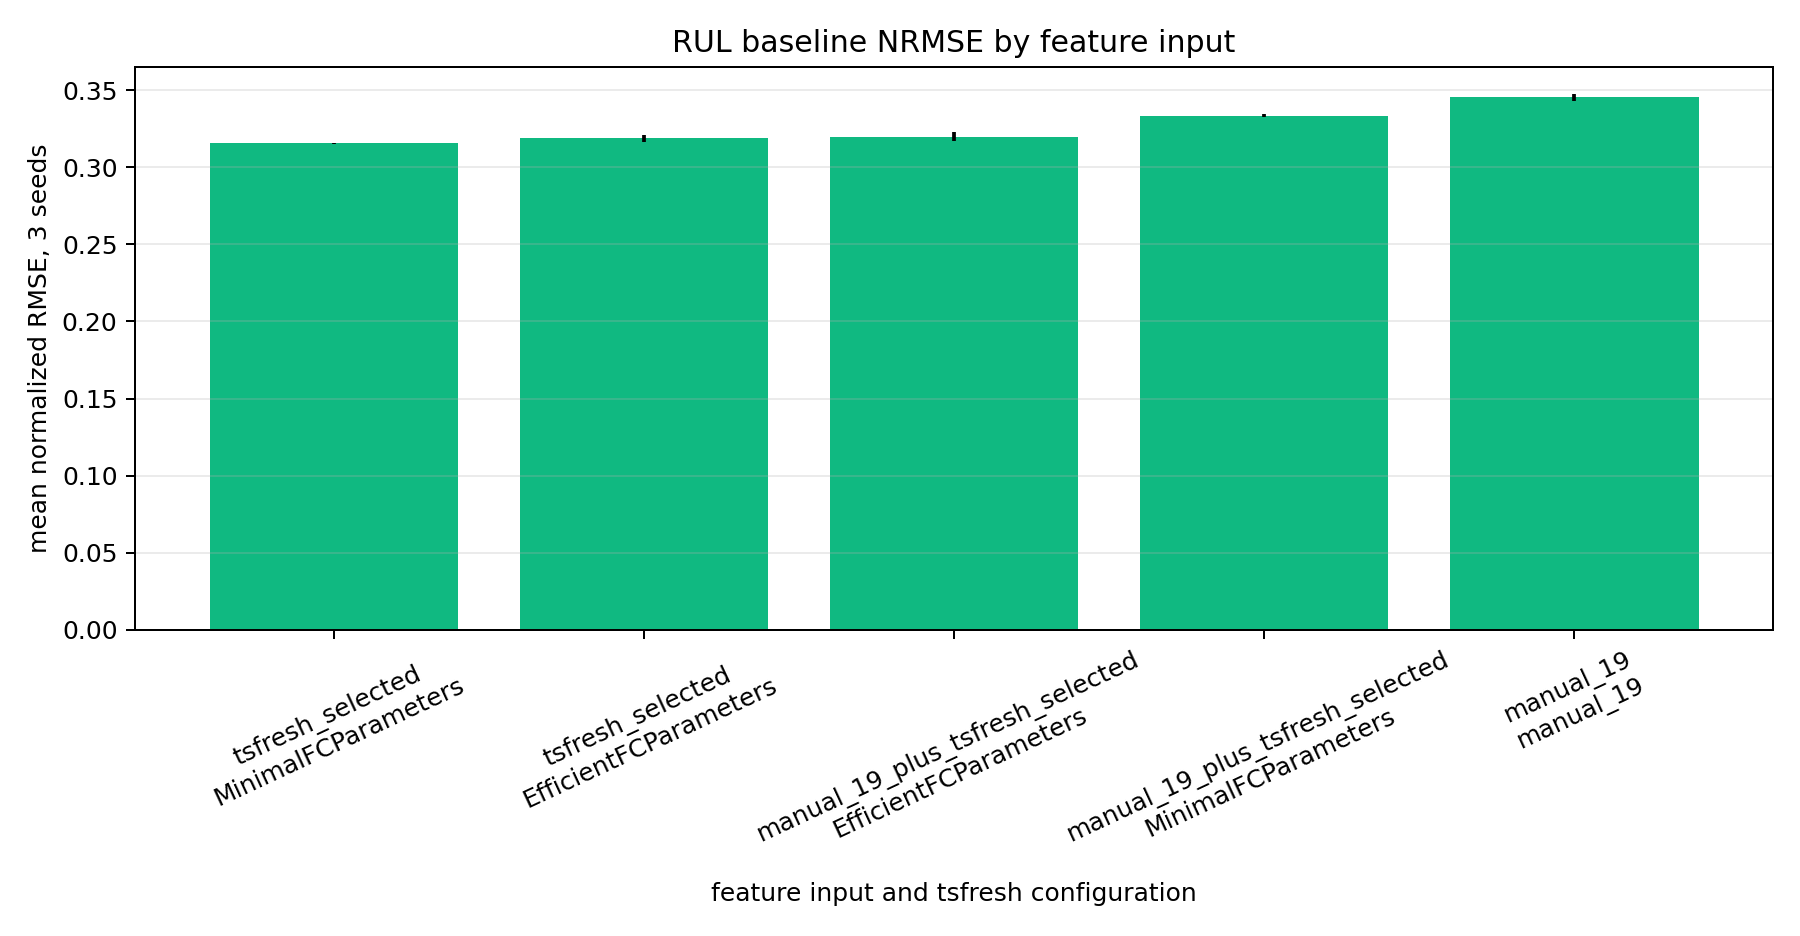
\includegraphics[width=0.85\textwidth]{docs/reproduction-evidence/tsfresh_rul_baseline_nrmse_comparison.png}
\caption{tsfresh 与手工特征 RUL baseline 对照}
\end{figure}

外部 AutoRUL、GNN RUL Benchmarking、Weibull KIML 已完成 source pin 和依赖 probe，但尚未在本项目环境跑出本地指标，因此不能宣称这些外部 SOTA 路线已复现完成。

\section{测试与质量保证}

\subsection{测试范围}

测试覆盖数据加载、特征构造、标签生成、模型 forward、训练 pipeline、预测模式、指标计算、notebook 示例、论文复现 workflow、metric-driven evidence 和 final materials alignment。当前全量测试数量为 59。

\begin{table}[H]
\centering
\caption{测试文件与覆盖重点}
\begin{tabularx}{\textwidth}{p{5.2cm}Y}
\toprule
测试文件 & 覆盖重点 \\
\midrule
\code{test\_data\_io\_and\_loaders.py} & XJTU/PHM2012 loader、采样元数据、温度通道、序列化。 \\
\code{test\_paper\_cnn\_lstm\_attention.py} & 19 维特征、CNN-LSTM-AM 结构、attention 和复现 workflow。 \\
\code{test\_paper\_xlstm\_transformer.py} & xLSTM-Transformer forward、真实数据检查、notebook 入口。 \\
\code{test\_prediction\_modes.py} & 滚动预测和 MC Dropout 不确定性估计。 \\
\code{test\_rul\_metrics.py} & RUL 回归指标、Huang Score、非对称惩罚。 \\
\code{test\_metric\_driven\_issue2\_evidence.py} & tsfresh、sktime、strict seed、external SOTA evidence。 \\
\code{test\_open\_source\_sota\_evidence.py} & SOTA target、gap 计算、RULSurv port evidence。 \\
\code{test\_examples\_notebooks.py} & 8 个示例 notebook 可执行。 \\
\bottomrule
\end{tabularx}
\end{table}

\subsection{实验输出证据}

训练和复现输出以文件形式保存，便于回查：

\begin{itemize}
  \item \code{history.csv}：记录 epoch 级训练/验证 loss 和 RMSE；
  \item \code{predictions.csv}：记录目标值、预测值和样本元数据；
  \item \code{metrics.json} 或 \code{comparison\_metrics.csv}：记录汇总指标；
  \item \code{attention\_weights.csv}：保留 attention 模型的权重输出；
  \item \code{docs/reproduction-evidence/*.csv}：保存正式复现实验摘要和补充证据。
\end{itemize}

\section{实现边界与风险}

当前项目应采用以下保守表述：

\begin{itemize}
  \item 已完成一条可复查的 RUL 预测流程，不应把正文全部称为生产级系统。
  \item 生存概率和失效概率是扩展能力，不能说成已与 RUL 主线同等充分验证。
  \item 两篇论文复现是结构、流程和指标体系复现，不是作者源码级逐行复刻。
  \item 正式训练已达到 50 epoch，但仍采用每轴承 96 快照抽样，不能替代全量训练。
  \item tsfresh 是自动特征分析旁证，不是核心性能突破。
  \item RULSurv row-level 协议复现和 held-out migration 必须分开解释。
  \item AutoRUL、GNN、Weibull KIML 等外部路线尚未产出本地指标，不能写成已完成复现。
\end{itemize}

\section{结论}

本项目从软件工程角度组织了工业轴承剩余寿命预测任务，形成了三条主要证据链。第一条是从真实数据文件到统一 \code{BearingEntity} 的数据链路；第二条是从振动快照到 19 维特征、RUL 标签和特征序列输入的建模链路；第三条是从真实训练到 \code{history.csv}、\code{predictions.csv}、指标表、测试报告和课程材料的验证链路。

结题阶段最稳妥的技术结论是：项目已经完成 RUL 回归预测主线，实现了数据接入、特征工程、模型训练、论文复现和测试验证；同时保留生存概率和失效风险的扩展接口。后续若继续完善，应优先扩大真实训练规模、补充更多随机种子和全量样本、融合温度信息，并为生存分析建立独立的数据构造、指标和可视化验收流程。

\section*{参考资料}
\addcontentsline{toc}{section}{参考资料}

\begin{enumerate}
  \item 项目 README：\code{README.md}。
  \item 项目 owner 分册：\code{docs/project-owner/}。
  \item 复现实验证据：\code{docs/reproduction-evidence/}。
  \item 结题报告与技术论文：\code{docx/final/md/12\_结题报告.md}，\code{docx/final/md/18\_项目技术论文.md}。
  \item Huang, W. et al. Life prediction method of rolling bearing based on CNN-LSTM-AM. \textit{Journal of Vibroengineering}, 2024.
  \item Jiang, R. et al. RUL Prediction Based on xLSTM-Transformer Neural Network for Rolling Element Bearings Under Different Working Conditions. \textit{Sensors}, 2026.
  \item Nectoux, P. et al. PRONOSTIA: An experimental platform for bearings accelerated degradation tests. IEEE PHM, 2012.
  \item XJTU-SY rolling element bearing accelerated life test dataset documentation.
\end{enumerate}

\end{document}
